\chapter{Background: Eclipse JDT and Jigsaw}\label{background2}

In order to construct structural generalizations describing the commonalities and differences between logged Java methods (LJMs), we need a concrete framework for constructing and manipulating abstract syntax trees (ASTs).  The Eclipse integrated development environment provides such a framework in its Java Development Tools (JDT) component.  The details of our implementation will depend on certain details of Eclipse JDT, so we describe those in Section~\ref{JDT}.

A framework exists for determining structural correspondences between ASTs, called Jigsaw \cite{2008:fse:cottrell}.  We build atop that work in order to create our anti-unifiers. We describe Jigsaw in Section~\ref{Jigsaw}.

\section{Eclipse JDT}\label{JDT}

The Eclipse Java Development Tools (JDT) framework provides APIs to access and manipulate Java source code via ASTs. An AST represents Java source code in a tree form, where the typed nodes represent instances of certain syntactic structures from the Java programming language.  Each node type (in general) takes a set of child nodes, also typed and with certain constraints on their properties.  Groups of children are named on the basis of the conceptual purpose of those groups; optional groups can be empty, which we can represent with the \NIL{} element. Thus, any Java source code can be represented as a tree of AST nodes. For example, the simple AST structure of two sample logged Java classes in Figures~\ref{ch3-ex1} an~\ref{ch3-ex2} is shown in Figure~\ref{fig:ast}

\begin{figure}[p]
\def\baselinestretch{1}
\begin{lstlisting}
public abstract class EBPlugin extends EditPlugin implements EBComponent {
    private Boolean seenWarning;

    protected EBPlugin() {
    }

    public void handleMessage(EBMessage message) {
        if(seenWarning) return;
        seenWarning = true;
        Log.log(Log.WARNING, this, getClassName() + " should extend EditPlugin not EBPlugin since it has an empty " + handleMessage());
    }
}
\end{lstlisting}
\caption{A Java class that uses a logging call. This will be referred to as Example 1.\label{ch3-ex1}}
\end{figure}

\begin{figure}[p]
\def\baselinestretch{1}
\begin{lstlisting}
public static class Wrapper implements ActionListener {
    private ActionContext context;
    private String actionName;

    public Wrapper(ActionContext context,  String actionName) {
        this.context = context;
        this.actionName = actionName;
    }

    public void actionPerformed(ActionEvent evt) {
        EditAction action = context.getAction(actionName);
        if(action == null) {
            Log.log(Log.ERROR, this, "Unknown action: " + actionName);
        }
        else
            context.invokeAction(evt, action);
    }
}
\end{lstlisting}
\caption{A Java class that uses a logging call. This will be referred to as Example 2.\label{ch3-ex2}}
\end{figure}

\begin{figure} [p]
  \centering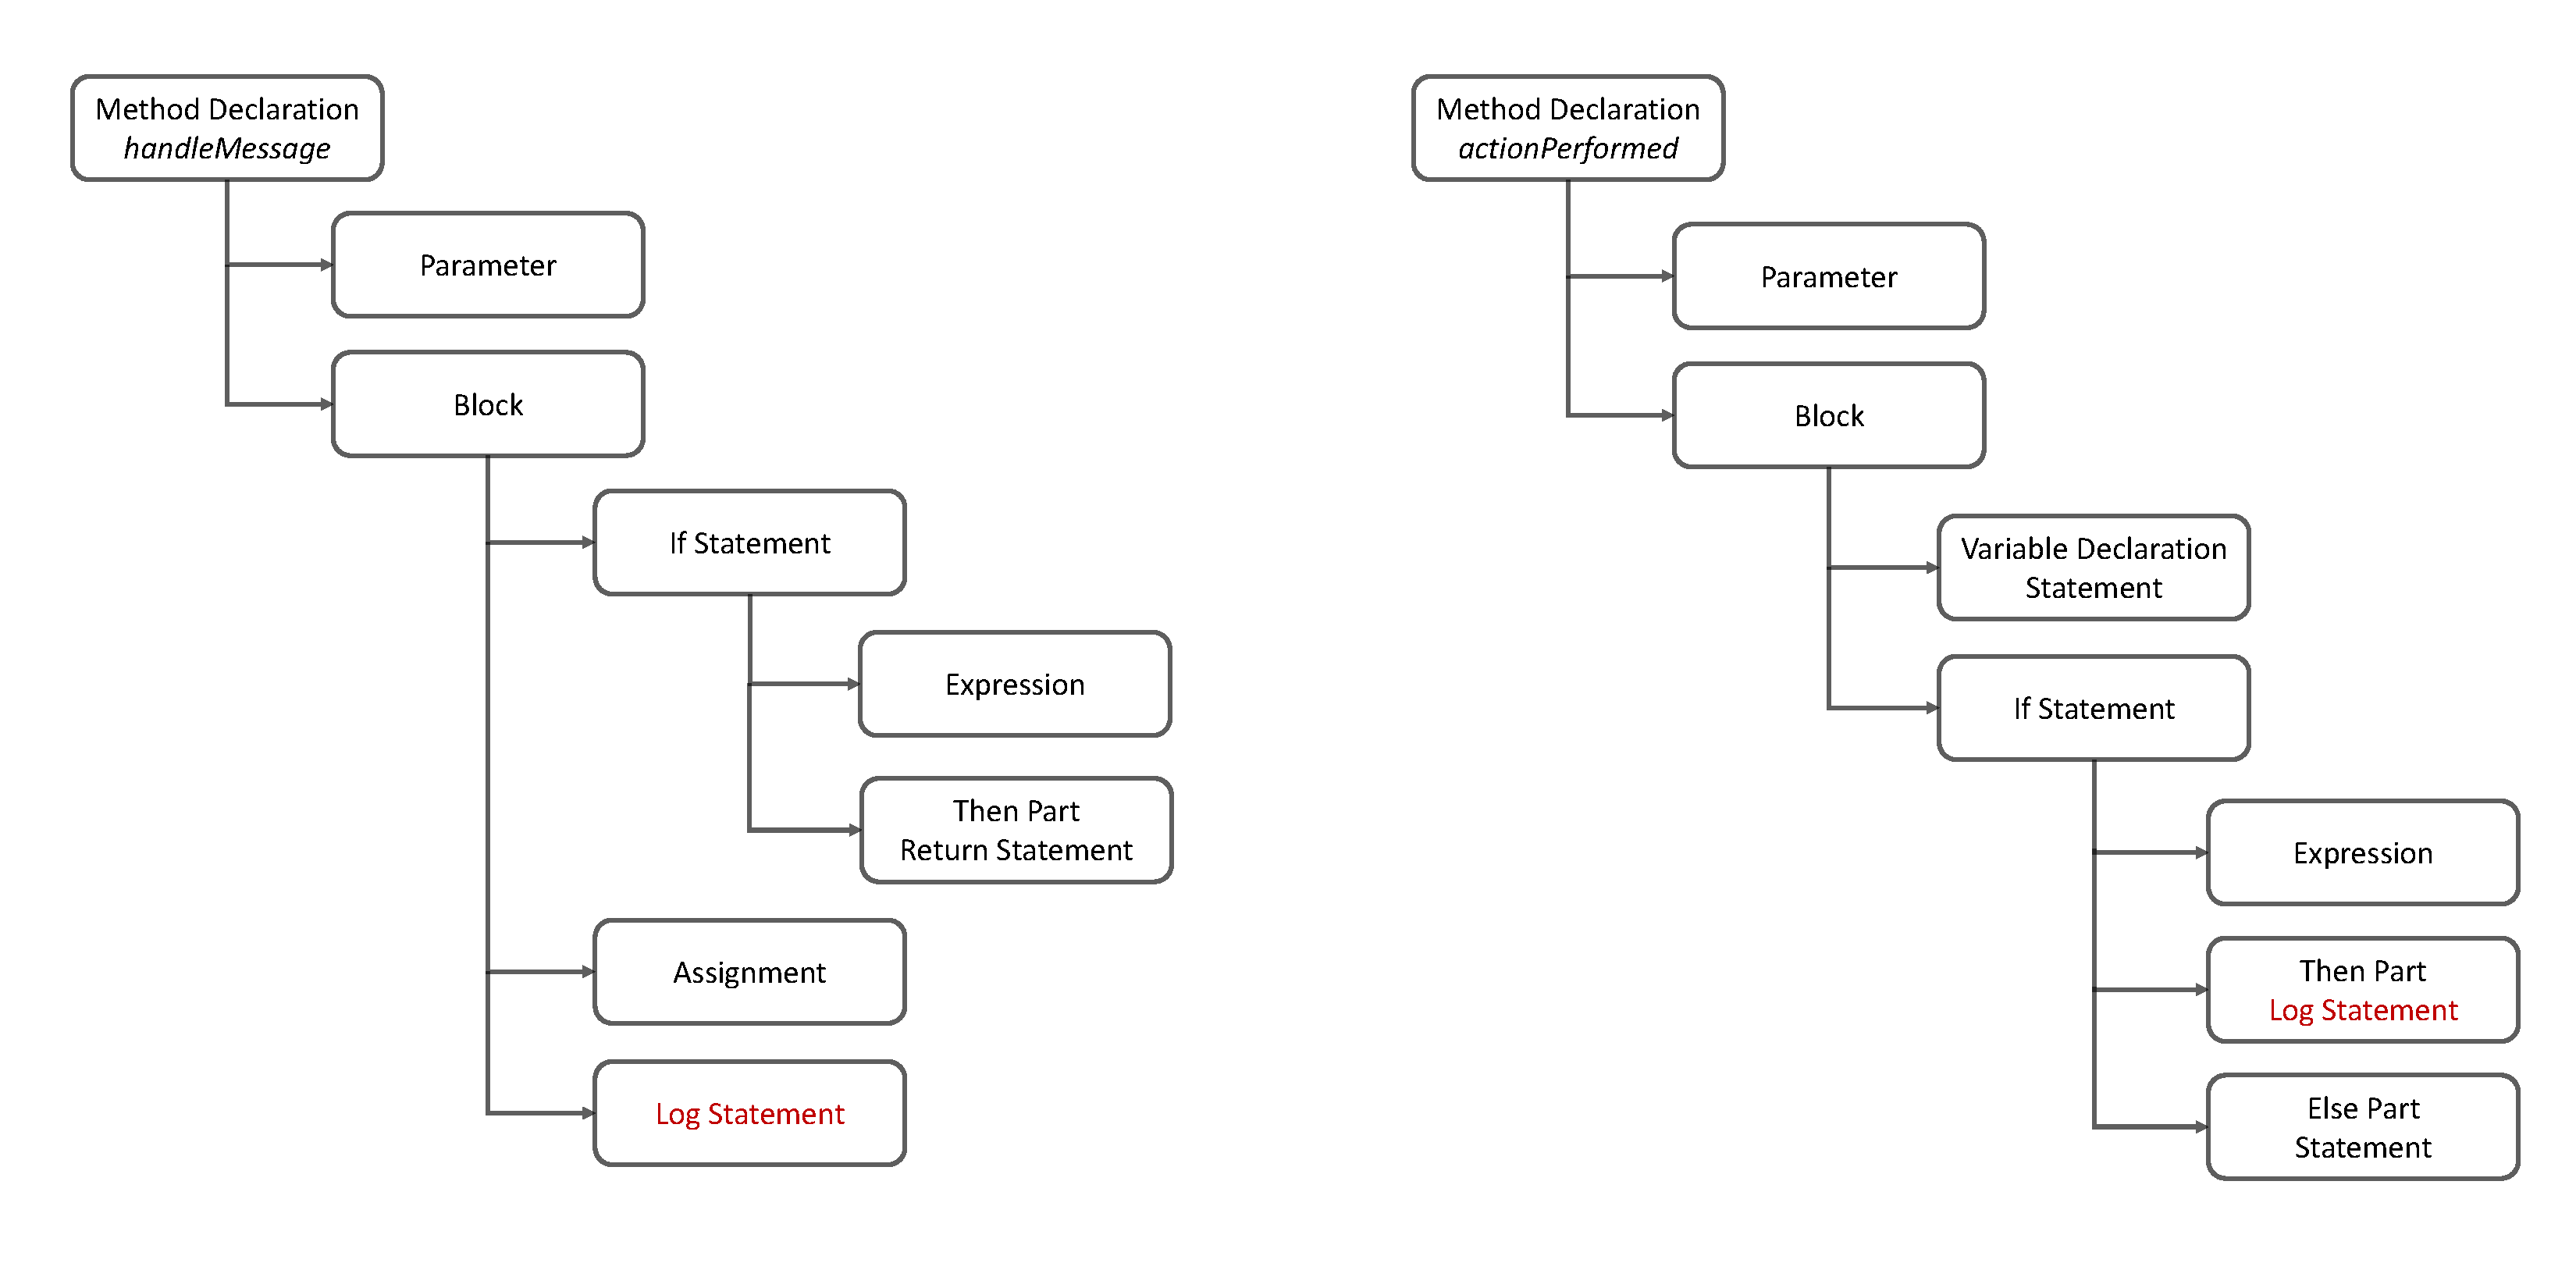
\includegraphics[width = \textwidth]{Drawing4/AST.pdf}
  \caption{Simple AST structure of examples in Figures~\ref{ch3-ex1} and~\ref{ch3-ex2}.}
  \label{fig:ast}
\end{figure}

In the JDT framework, structural properties of each AST node can be used to obtain specific information of the Java element that it represents. These properties are stored in a map data structure that associates each property to its value; this data is divided into three types:
\begin{itemize} [leftmargin=0.7in]
\item \textit{Simple structural properties:} These contain a simple value which has a primitive or simple type or a basic AST constant (e.g., identifier property of a name node whose value is a String).  For example, all the \textit{Identifier} nodes in Figure~\ref{fig:java-example-ast} fall in this case; each references an instance of \code{String} representing the string that constitutes the identifier.
\item \textit{Child structural properties:} These involve situations where the value is a single AST node (e.g., name property of a method declaration node).  For example, the \textit{ClassDeclaration} node in Figure~\ref{fig:java-example-ast} has a single child that represents its name as an \textit{Identifier} node; this would be a child structural property.
\item \textit{Child list structural properties}: These involve situations where the value is a list of child nodes.  For example, the \textit{ClassDeclaration} node in Figure~\ref{fig:java-example-ast} can possess multiple \textit{Modifier}s; these are recorded in the \textit{ClassDeclaration} as a child list structural property.
\end{itemize}

As an example, the ASTs of the logging calls at line~10 of Figure~\ref{ch3-ex1} and line~13 of Figure~\ref{ch3-ex2} can be represented respectively as:
\begin{itemize} [leftmargin=0.7in]
%\RW{These ASTs were messed up.  I fixed them according to what the code says.}
%\item \textit{expression(expression(Log), name(log), arguments(leftoperand(message), +, rightoperand(" is empty"), qualifier(Log), name(WARNING)))}
%\item \textit{expression(expression(Log), name(log), arguments(leftoperand(actionName),\\+, rightoperand("is an unknown action"), qualifier(Log), name(WARNING)))}
\item \textit{MethodCall}(\\
\hspace*{1em}\textit{QualifiedName}(\code{Log}, \textit{Identifier}(\code{log})),\\
\hspace*{1em}\textit{Arguments}(\\
\hspace*{2em}\textit{QualifiedName}(\code{Log}, \mbox{\textit{Identifier}(\code{WARNING})}),\\
\hspace*{2em}\textit{ThisExpression}(),\\
\hspace*{2em}\textit{AdditionExpression}(\\
\hspace*{3em}\textit{MethodInvocation}(\textit{Identifier}(\code{getClassName}), \textit{Arguments}()),\\
\hspace*{3em}\textit{StringLiteral}(\code{" should extend EditPlugin not EBPlugin since it has an empty "}),\\
\hspace*{3em}\textit{MethodInvocation}(\textit{Identifier}(\code{handleMessage}), \textit{Arguments}()))))\\
\item \textit{MethodInvocation}(\\
\hspace*{1em}\textit{QualifiedName}(\code{Log}, \textit{Identifier}(\code{log})),\\
\hspace*{1em}\textit{Arguments}(\\
\hspace*{2em}\textit{QualifiedName}(\code{Log}, \mbox{\textit{Identifier}(\code{ERROR})}),\\
\hspace*{2em}\textit{ThisExpression}(),\\
\hspace*{2em}\textit{AdditionExpression}(\\
\hspace*{3em}\textit{StringLiteral}(\code{"Unknown action: "}),\\
\hspace*{3em}\textit{Identifier}(\code{actionName}))))\\
\end{itemize}

\section{The Jigsaw framework}\label{Jigsaw}
The Jigsaw tool was developed by \citet{2008:fse:cottrell} to determine the structural correspondences between two Java source code fragments through the application of higher-order anti-unification modulo equational theories such that one fragment can be integrated to the other one for small-scale code reuse. Jigsaw could help determine potential candidate structural correspondences between AST nodes of logged Java classes by producing an augmented form of AST, called a \emph{correspondence AST} (CAST), where each node holds a list of candidate correspondence connections between the two structures, each implicitly representing an anti-unifier. Jigsaw also provides a measure of structural similarity to indicate how similar the nodes involved in each correspondence connection are. The Jigsaw similarity function relies on structural correspondence along with simple knowledge of semantic equivalences supported by the Java language specification. It returns a value in $[0, 1]$ where zero indicates complete lack of similarity and one indicates perfect similarity. In addition, several semantical heuristics are used to improve the accuracy of similarity measurement by allowing the comparison of AST nodes that are not syntactically identical but are semantically related to each other.

For example, the similarity between names of AST nodes is measured using a normalized computation based on the length of the longest common substring. The comparison of \code{int} and \code{long} types is another example, where an arbitrary value of 0.5 is defined as the similarity value as they are not syntactically identical but are semantically related. In addition, the Jigsaw framework also detects the structural correspondence between  \code{for}-, enhanced-\code{for}-, \code{while}-, and \code{do}-loop statements; and \code{if} and \code{switch} conditional statements. As an example, Figure~\ref{fig:meth-ast-1} shows the structural correspondence connections created by Jigsaw between the AST nodes of Examples 1 and 2 along with the similarity value for each correspondence connection.

\begin{figure} [H]
  \centering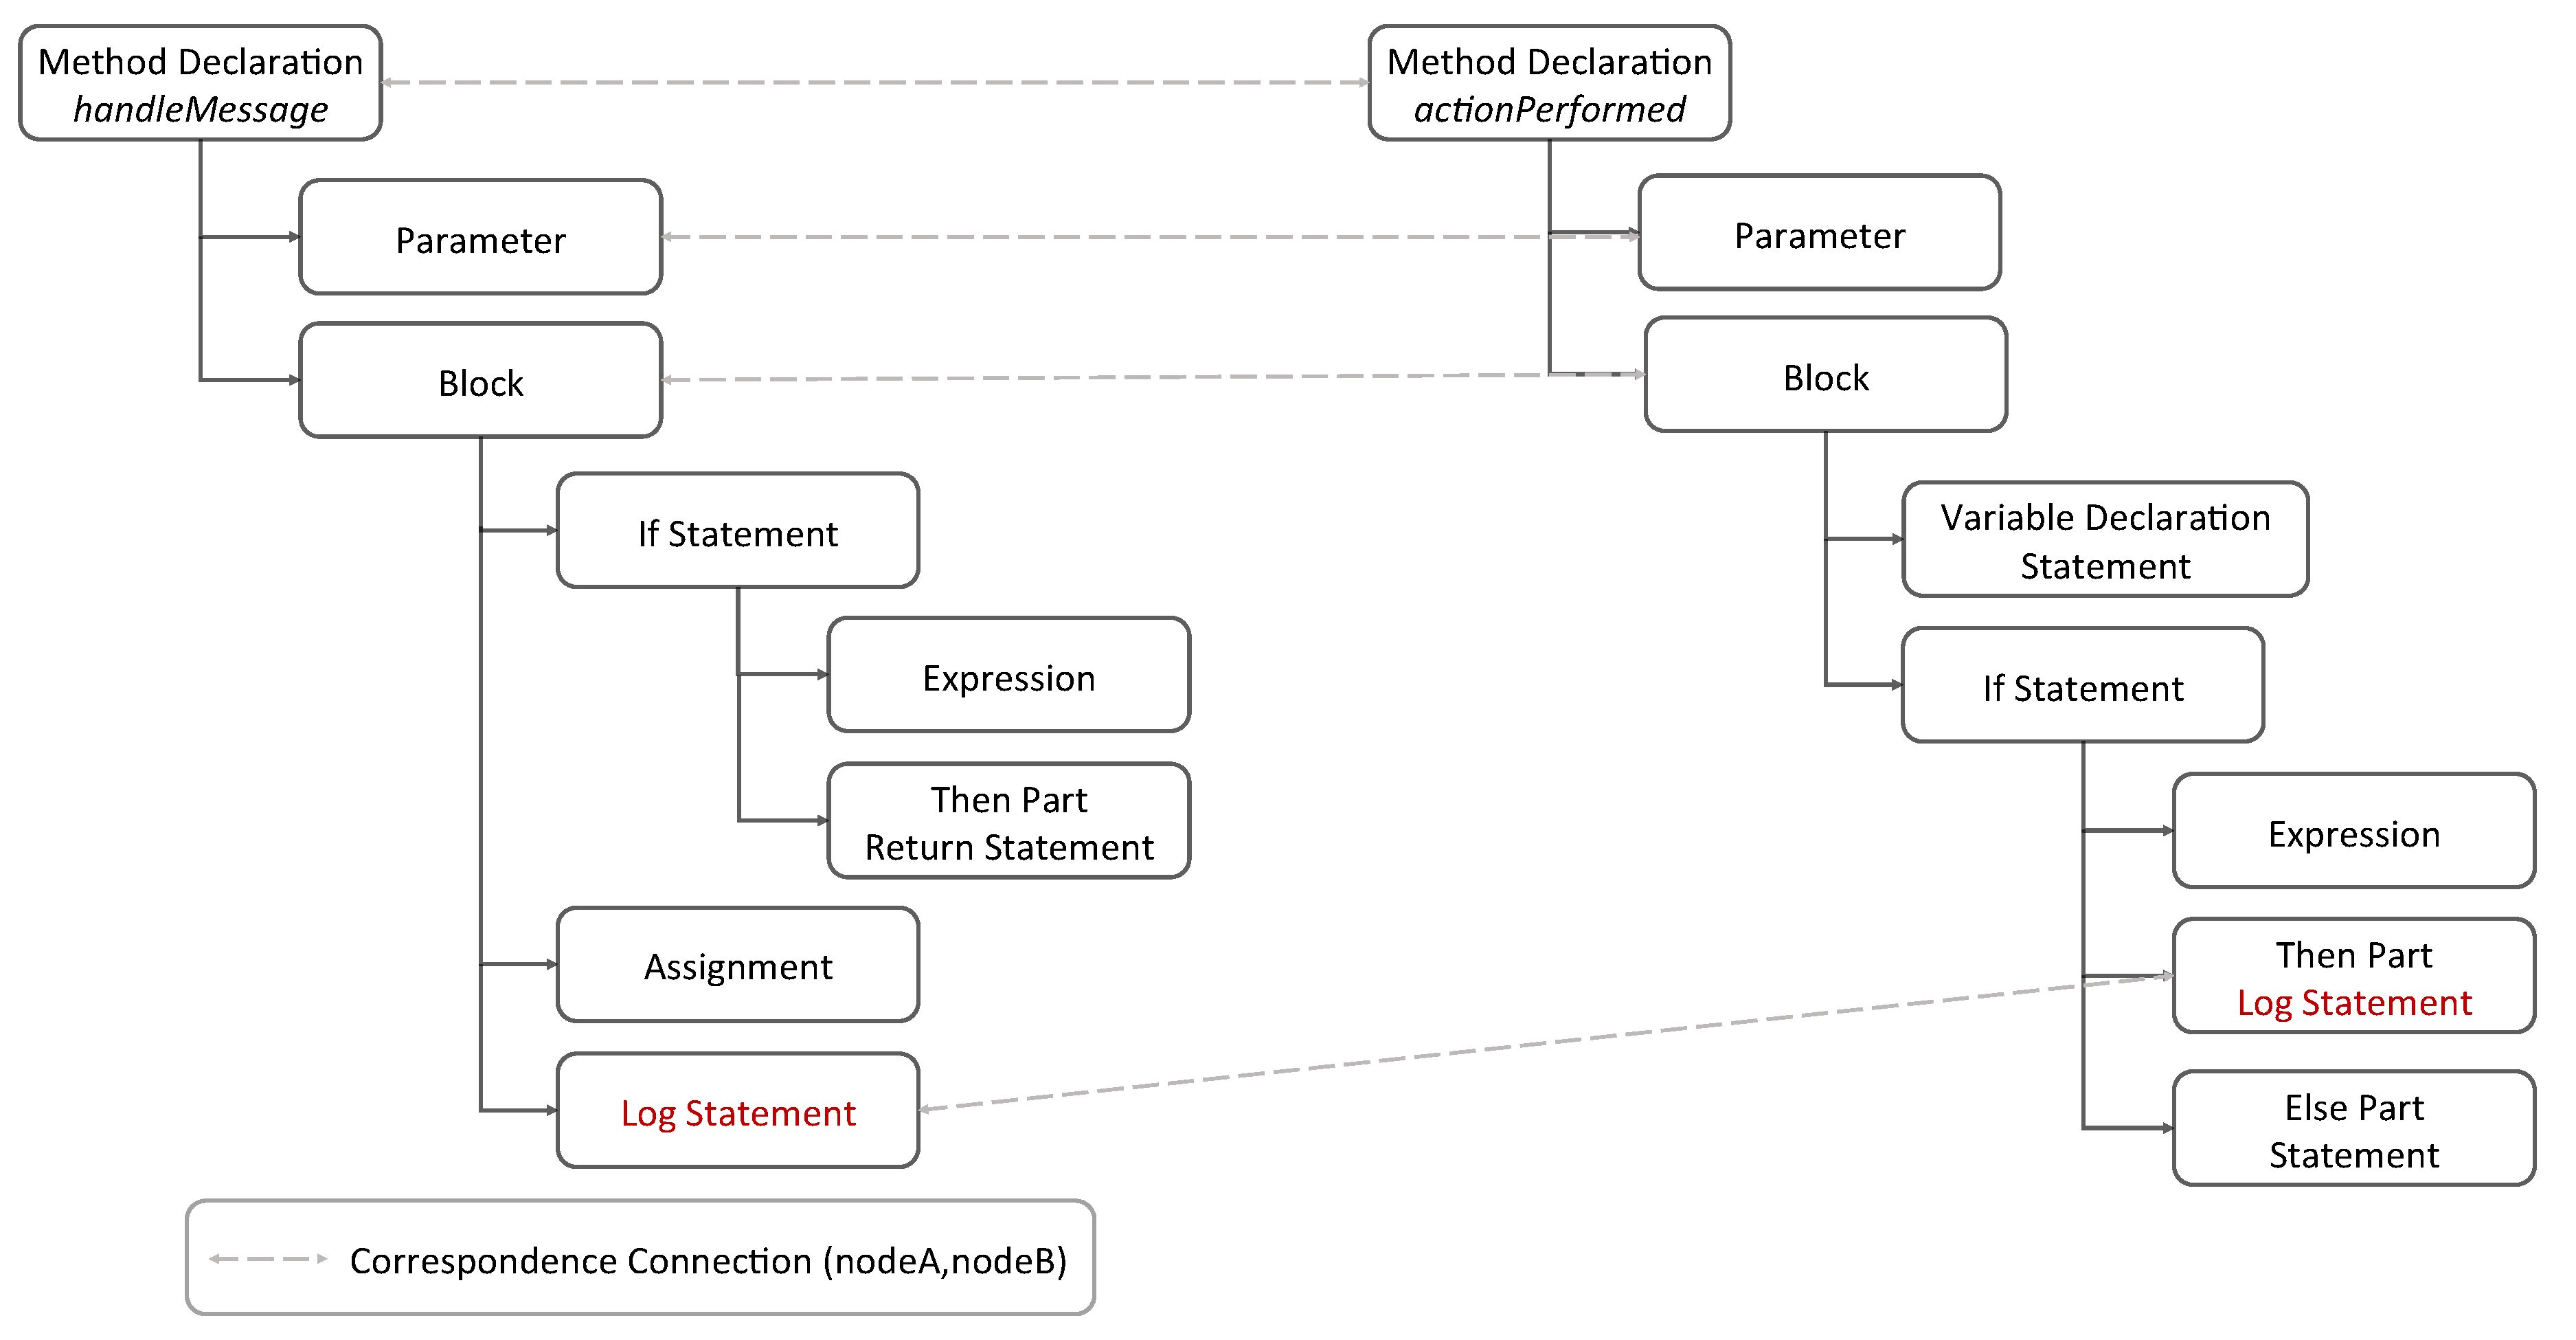
\includegraphics [width = \textwidth]{Drawing4/FirstCorr.pdf}
  \caption{Simple CAST structure of examples in Figures~\ref{ch3-ex1} and~\ref{ch3-ex2}. The links between AST nodes indicate structural correspondence connections created by the Jigsaw framework along with the similarity value.}
  \label{fig:meth-ast-1}
\end{figure}

However, the Jigsaw tool does not suffice to construct an anti-unifier that is the best fit to our application. In addition, the Jigsaw similarity function does not measure the similarity of two logged Java classes with a focus on logging calls, which is needed in our context. To address these issues, we should develop a greedy selection algorithm to approximate the best anti-unifier by determining the best correspondence for each node. In the following chapter, we will discuss our approach to construct structural generalizations and our implementation by means of the higher-order anti-unification modulo theories and the Jigsaw framework.

\section{Summary}  \label{summary}
\RW{Redo}